% This is samplepaper.tex, a sample chapter demonstrating the
% LLNCS macro package for Springer Computer Science proceedings;
% Version 2.20 of 2017/10/04
%
\documentclass[runningheads]{llncs}
%
\usepackage{graphicx}
% Used for displaying a sample figure. If possible, figure files should
% be included in EPS format.
%
% If you use the hyperref package, please uncomment the following line
% to display URLs in blue roman font according to Springer's eBook style:
% \renewcommand\UrlFont{\color{blue}\rmfamily}
\usepackage{hyperref} % to handle underscores in url 

\begin{document}
%
\title{Corridor Coupling Between Intersection Management Zones for Site-Wide Motion Co-ordination of an Autonomous Vehicle Fleet   
\thanks{Supported by the Engineering and Physical Sciences Research Council through a full time Doctoral Training Partnership Studentship - Institute for Transport Studies - EPSRC Project Reference 2383174 and in a Combined Award in Science and Engineering partnership with Guidance Automation Limited. 
 }}
%
\titlerunning{Corridor Coupling Between Intersection Management Zones}
% If the paper title is too long for the running head, you can set
% an abbreviated paper title here
%
\author{Edward Derek Lambert\inst{1}\orcidID{0000-0002-2297-0441} \and
David Watling  \inst{1}\orcidID{0000-0002-6193-9121} \and
Richard Romano\inst{1}\orcidID{0000-0002-2132-4077}}
%
\authorrunning{ED. Lambert et al }
% First names are abbreviated in the running head.
% If there are more than two authors, 'et al.' is used.
%
\institute{Institute for Transport Studies, University of Leeds, 34-41 University Road, Leeds, West Yorkshire LS2 9JT UK
\email{\{tsedl, D.P.Watling, R.Romano\}@leeds.ac.uk}
\url{https://environment.leeds.ac.uk/transport} }
%
\maketitle              % typeset the header of the contribution
%
\begin{abstract}
The abstract should briefly summarize the contents of the paper in
150--250 words.

\keywords{Modelling \and  Analysis \and Safety Validation \and Robot Communication \and Autonomous Vehicles \and Collective Field Robotics}
\end{abstract}
%
%
%
%\subsection{A Subsection Sample}
%Please note that the first paragraph of a section or subsection is
%not indented. The first paragraph that follows a table, figure,
%equation etc. does not need an indent, either.
%
%Subsequent paragraphs, however, are indented.
%
\section{Introduction}

Collaborative mobile robots are being adopted widely in distribution centres and factories to increase efficiency and reduce operating costs \cite{Azadeh2019}. Models indicate they are most beneficial to e-commerce pick-pack-and-ship warehouses where the existing pick density is low \cite{Meller2018}. In this situation, adding a number of automated trolleys to ferry items back to the packing station can reduce the time pickers spend walking backwards and forwards, freeing them up to pick more items.

\begin{figure}[htbp]
\centerline{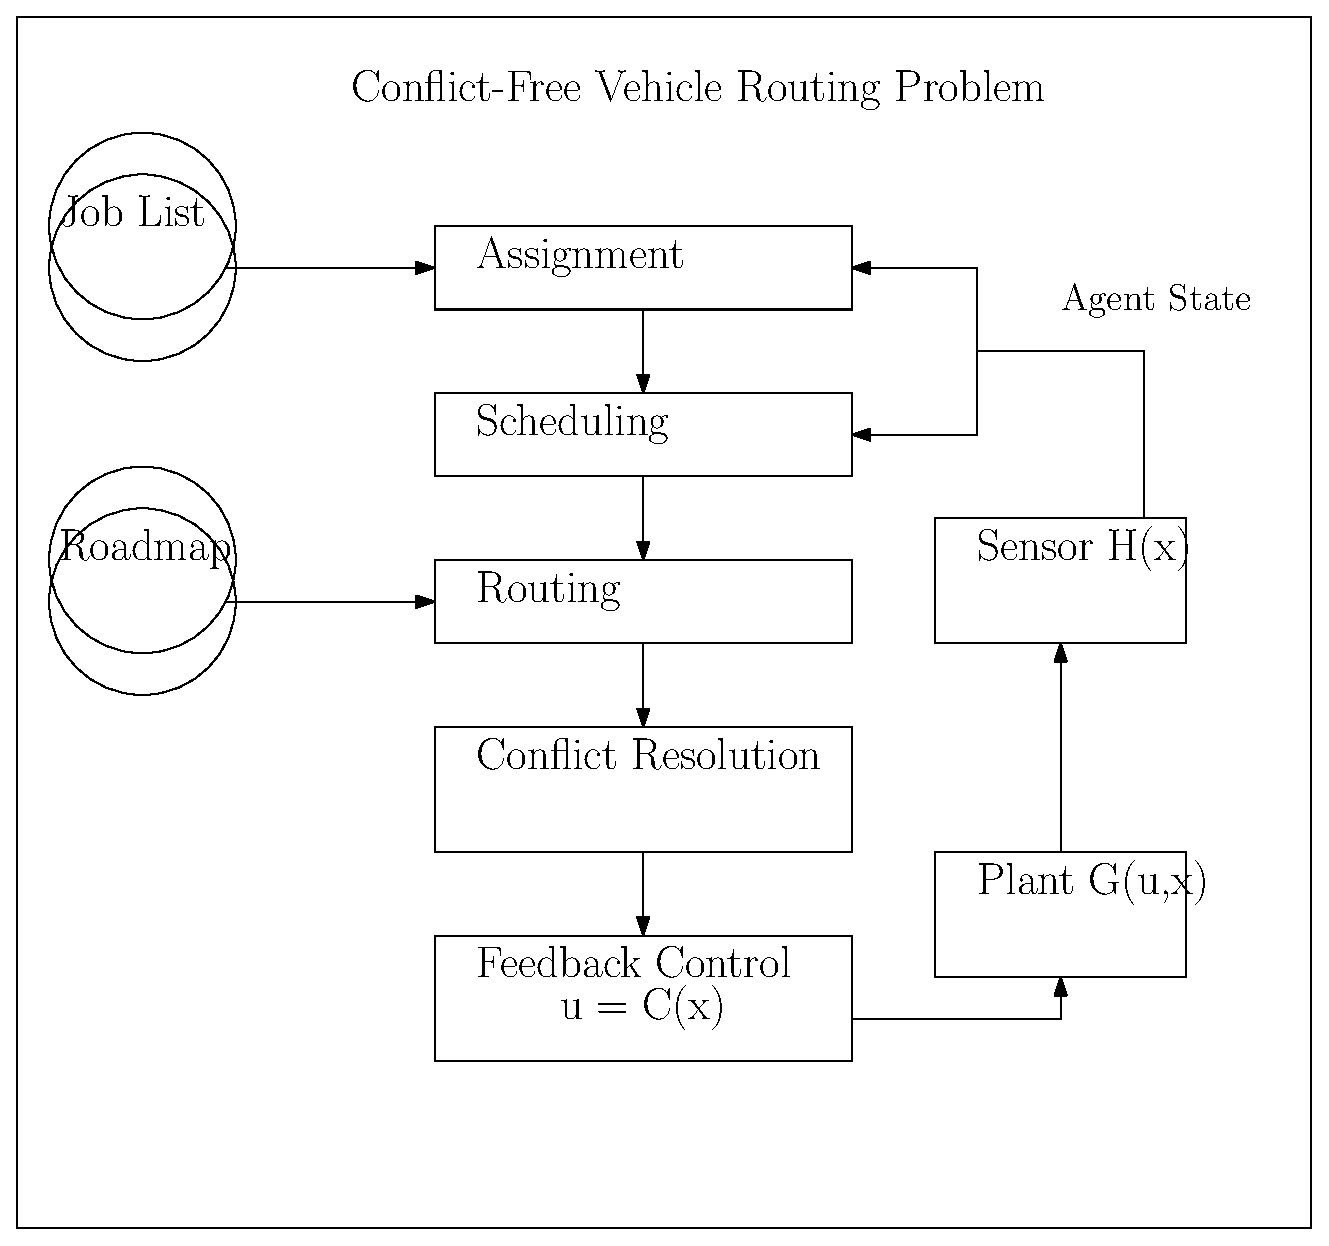
\includegraphics[width=0.7\linewidth]{dcfvrp_logical_blocks.eps}}
\caption{Possible logical division of Fleet Control tasks}
\label{fig:logical_blocks}
\end{figure}
A roadmap-based mobile robot system is a frequently used in material handling, although recently more advanced vehicles are able to take on more of the decision making, and in some cases plan their motion without supervision making them Autonomous Mobile Robots (AMR) \cite{Fragapane2021}. The fleet operator is likely to desire the most items transported in a set time, given a fixed amount of floor space. This leads to a key objective of maximum throughput for the whole site or equivalently minimum makespan \cite{Lamballais2017}.    

A fully decentralized and complete solution for controlling a fleet of autonomous mobile robots, not restricted to guide paths is given by Draganjac et al \cite{Draganjac2020}. Planning is divided into a topological layer and a more detailed private zone, a dense lattice of smooth radial polynomial paths. Live-locks are avoided as topological plans are fixed so AMR continue along the shortest topological path. Conflicts are handled and the lower layer with prioritized local negotiations in private zones. The two layers address the Routing and Conflict Resolution components of the overall fleet control problem shown in Figure \ref{fig:logical_blocks}. Deadlocks are ruled out as each local zone contains an avoidance state reachable within one move. There is also an explicit circular-wait detection procedure within the published algorithm. Results for 50 vehicles in simulation demonstrate the scalability of this approach, where a centralized algorithm might require many seconds to compute a set of safe trajectories for 10 vehicles. 

One drawback of decentralized methods comes from the time spent negotiating at each intersection. Experiments show an average negotiation time of several seconds, and a number of conflicts increase with the number of vehicles \cite{Draganjac2020}. Reducing the number of negotiations is the motivation for the intersection control based solution described by Digani et al \cite{Digani2019}. The test environment used fixed guide paths, but modern AMR resemble autonomous vehicles which may one day operate on public roads, for which Autonomous Intersection Management has been well studied. 

Car-following conflicts are resolved by the centralized routing algorithm in the reference `Full-Control' Fleet Adapter available within the Open Source Robotic Foundation's Robotic Middleware Framework (RMF) as of May 2021 \cite{Vijay2021}. This is consistent with wider industry practice for roadmap-based systems reported in \cite{Fragapane2021}. Another notable adapter is the MiR 100 Fleet adapter, which is used to control a fleet of  MiR100 AMRs, currently in operation at an Airbus wing factory amongst other sites. The degree of autonomy is sufficiently high that a highway code has been proposed to govern the motion \cite{Liaqat2019}. The adapter appears to be a thin wrapper around the default RMF Fleet Adapter Python library, and chiefly serves to translate the DDS messages used in ROS2 \cite{Eros2019} to the bespoke REST interface used by the MiR100 Robots \cite{Grey2021}. For this reason it is likely to be roadmap-based with a centralized controller capable of conflict-free routing with a modified A* algorithm. Reported fleet behaviour seem to corroborate this suggestion, at least in the 2019 release \cite{Liaqat2019}.

With roadmap-reservation based collision avoidance, the following vehicle must wait until the leader has completely vacated a private zone before the follower may progress. This behaviour is convenient because it extends safely to crossing traffic without modification. The concept is simple and offers flexibility as the size of the private zone can be tuned to achieve closer spacing where desired, for example in \cite{Walenta2017} there are two zone sizes depending on whether the direction of travel is the same or not. This is a good approximation to car-following, and notable for its decentralized design too. A follow up study to investigate the added messaging overhead and potential for negotiation delay, notwithstanding, this solution could offer throughput advantages.

Research in to AIM for near future Autonomous Vehicles offers an alternative vision for multi vehicle collision avoidance, seemingly suitable for recent AMR with a high level of autonomy. A recent review is given by Zhong et al \cite{Zhong2020}. In in some car-following conflicts are explicitly excluded such as \cite{Yao2020}, perhaps because autonomous vehicles suitable for operation on public roads are assumed to execute this function using their own sensors, perhaps in a similar way to the Adaptive Cruise Control assistance feature available in many production vehicles. Even so, the impact of interactions between vehicles are likely to be important to ensure the safe operation across the intersection. For example, even smart AMR who can overtake a lead vehicle if the AIM requests a different arrival order may well take longer to arrive, traverse a different path, or even be completely prevented from doing so by opposing traffic or vary narrow aisles. 

Zhong et al \cite{Zhong2020} includes a summary table of AIM approaches, which indicates that little attention has been given to the corridor coordination layer.  One of the few works addressing interactions between intersection zones is \cite{Du2018} which uses a 3-layer hierarchy where the manager of each intersection sends the average traffic density to its neighbours, chooses speeds within its zone of influence to minimize deviation from average road velocity, subject to the constraint that conflicts are avoided in the single zone spanning the intersection. 

The AIM* interface is described in \cite{Levin2017} for an isolated intersection. The interface for quadratic programming formulation for industrial robots described by Digani et al \cite{Digani2019} is similar.In this work multiple intersection zones are coupled to span the entire roadmap. Every place where two lanes intersect in the roadmap is identified and nearby elementary conflicts are collected into an conflict zone. The intersection manager for one zone only has authority over approaching vehicles, those within the intersection and departing can no longer be controlled, but their state is used as a constraint on the following vehicles. 

A vehicle departing one intersection is by definition approaching the next one, and new speeds instructions should be received as soon as communication with the next Intersection Manager can be established. As the speed of a departing vehicle is set by the next Intersection Manager, and the position of that vehicle forms a constraint on the solution to the speed of approaching vehicles computed by the previous intersection it could be argued that car-following behaviour is the fundamental mechanism for coupling intersection zones. Car-following in \cite{Digani2019} is based on roadmap reservation, reflecting the state of practice in industrial robotics. This leads to constraints that one vehicle cannot enter a roadmap segment, until the preceding one has departed. Provided the segments chosen are long enough, this provides guaranteed safe behaviour. In many cases it will be overly conservative, especially when one vehicle is following another at a similar speed. As both are in motion, in the same direction they can follow each other much closer than the braking distance either vehicle would need to stop for a stationary obstacle.

Other works have investigated the car-following behaviour \cite{Bichiou2019} using the RPA model, which accounts for vehicle dynamic limitations. Only an isolated intersection is modelled, but if it were used for Corridor Co-ordination it should be less conservative than roadmap reservation. The guarantees of correct behaviour need to be considered carefully as they could break down in some situations, such as those examined by \cite{Du2020}.


Using AIM to guarantee intersection safety, there is an opportunity to improve throughput by following more closely. The remaining research questions of interest to improve decentralized control of mobile robot fleets are:\\
1.  What are the performance implications of a conflict avoidance scheme based on platooning and AIM? \\
2. What are the implication for Stability/Correctness corridor coordination is used to extend this across a whole site? \\
3.  What is the impact on makespan in high traffic?\\










\section{Method}
As the conflict resolution is a safety critical function of an AGV fleet we need high confidence that it will perform correctly in all foreseeable situations, and shows some befit to performance before it is worth testing with hardware in the loop. The Robot Operating System library and associated Gazebo rigid body dynamic simulator are open source tools specifically designed to reduce the gap between numerical simulation and hardware tests. There is also a wide variety of open source software components which represent the state of practice and in some cases the state of the art. 
\begin{figure}[htbp]
\centerline{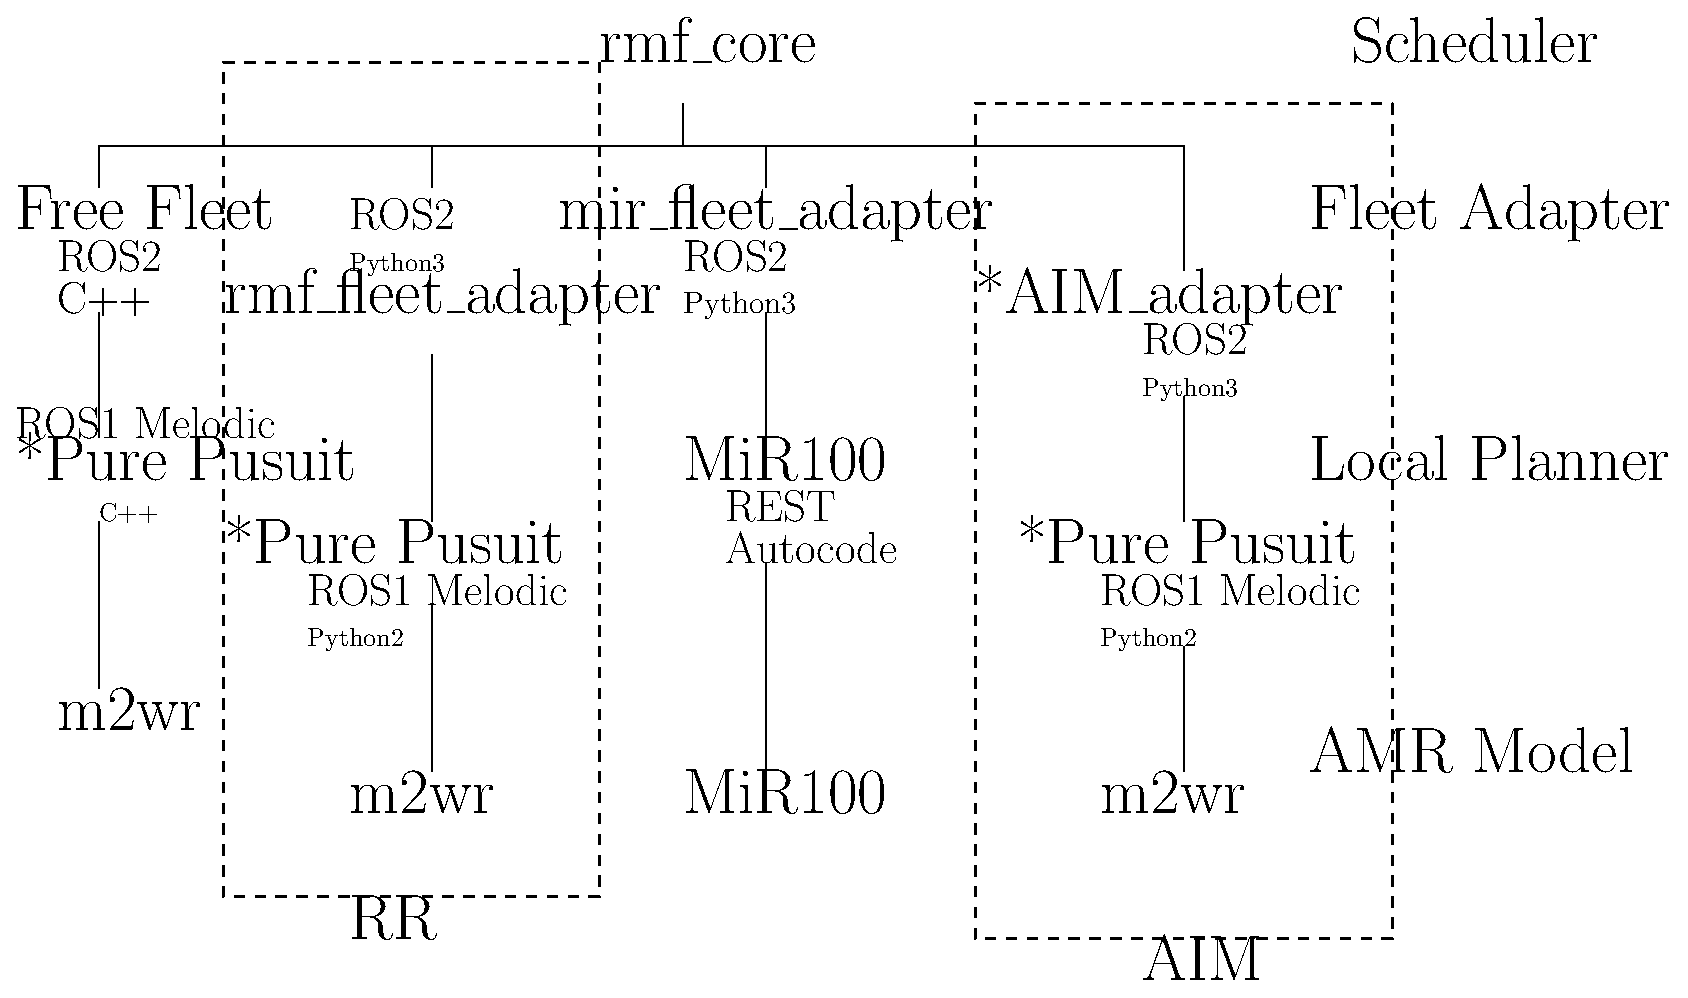
\includegraphics[width=0.7\linewidth]{ros2_fleet_options.eps}}
\caption{Different combinations of software packages to solve the Fleet Scheduling, and Conflict Free Routing problem. Bespoke implementations are marked with an asterisk. The selected stacks for comparison, labelled RR and AIM are enclosed in dashed boxes.}
\label{fig:ros2_fleet_options}
\end{figure}
We have identified several combinations of packages which would be sufficient to control a fleet of 50 AMR in a dynamic simulation of a warehouse environment, to complete a list of 500 movement tasks in a fixed order. There were several possible combinations as shown in Figure \ref{fig:ros2_fleet_options}. The tasks consist of a pick location and a drop location within the roadmap, which is known a priori. Each task can be be completed by any AMR. The load capacity is one unit, and all items take up one unit space, so there is no opportunity for tour planning, carrying out multiple picks before a drop. All AMR begin in random locations, in the empty state and never leave the simulation at any time.  

  
\section{Numerical Simulation Results}
\section{Concluding Remarks and Further Work}  
%\subsubsection{Sample Heading (Third Level)} Only two levels of
%headings should be numbered. Lower level headings remain unnumbered;
%they are formatted as run-in headings.
%
%\paragraph{Sample Heading (Fourth Level)}
%The contribution should contain no more than four levels of
%headings. Table~\ref{tab1} gives a summary of all heading levels.
%
%\begin{table}
%\caption{Table captions should be placed above the
%tables.}\label{tab1}
%\begin{tabular}{|l|l|l|}
%\hline
%Heading level &  Example & Font size and style\\
%\hline
%Title (centered) &  {\Large\bfseries Lecture Notes} & 14 point, bold\\
%1st-level heading &  {\large\bfseries 1 Introduction} & 12 point, bold\\
%2nd-level heading & {\bfseries 2.1 Printing Area} & 10 point, bold\\
%3rd-level heading & {\bfseries Run-in Heading in Bold.} Text follows & 10 point, bold\\
%4th-level heading & {\itshape Lowest Level Heading.} Text follows & 10 point, italic\\
%\hline
%\end{tabular}
%\end{table}
%
%
%\noindent Displayed equations are centered and set on a separate
%line.
%\begin{equation}
%x + y = z
%\end{equation}
%Please try to avoid rasterized images for line-art diagrams and
%schemas. Whenever possible, use vector graphics instead (see
%Fig.~\ref{fig1}).
%
%\begin{figure}
%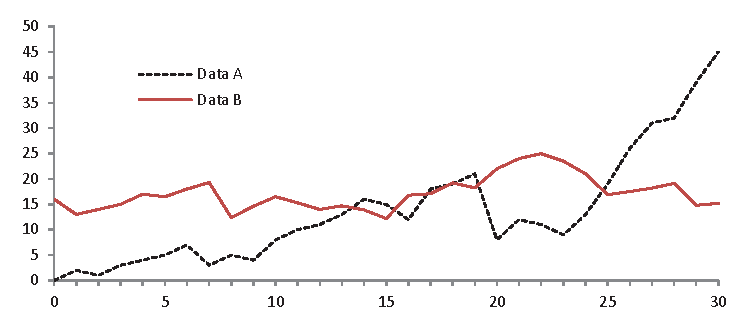
\includegraphics[width=\textwidth]{fig1.eps}
%\caption{A figure caption is always placed below the illustration.
%Please note that short captions are centered, while long ones are
%justified by the macro package automatically.} \label{fig1}
%\end{figure}
%
%\begin{theorem}
%This is a sample theorem. The run-in heading is set in bold, while
%the following text appears in italics. Definitions, lemmas,
%propositions, and corollaries are styled the same way.
%\end{theorem}
%%
%% the environments 'definition', 'lemma', 'proposition', 'corollary',
%% 'remark', and 'example' are defined in the LLNCS documentclass as well.
%%
%\begin{proof}
%Proofs, examples, and remarks have the initial word in italics,
%while the following text appears in normal font.
%\end{proof}
%For citations of references, we prefer the use of square brackets
%and consecutive numbers. Citations using labels or the author/year
%convention are also acceptable. The following bibliography provides
%a sample reference list with entries for journal
%articles~\cite{ref_article1}, an LNCS chapter~\cite{ref_lncs1}, a
%book~\cite{ref_book1}, proceedings without editors~\cite{ref_proc1},
%and a homepage~\cite{ref_url1}. Multiple citations are grouped
%\cite{ref_article1,ref_lncs1,ref_book1},
%\cite{ref_article1,ref_book1,ref_proc1,ref_url1}.
%
% ---- Bibliography ----
%
% BibTeX users should specify bibliography style 'splncs04'.
% References will then be sorted and formatted in the correct style.
%
\bibliographystyle{splncs04}
\bibliography{taros_references}

\end{document}
